Micro Air Vehicle Link is a lightweight header-only protocol used in the bidirectional communications between drones and a Control Ground Station (GCS). In general, the GCS sends commands to control the drone and the drone sends its status information in return. It is a binary telemetry protocol designed for resource-constrained systems and bandwidth-constrained links. Nowadays MAVLink is deployed in two major versions: v1.0 and v2.0, which is backwards-compatible. 
%[https://mavlink.io/en/protocol/overview.html]

MAVLink messages have defined formats in order to be consistent between the systems that use the protocol. These formats can be found in an XML file and can be converted to other languages formats, as C/C++ or Python, using a code generator. Writing a new definition in the XML enables to add new messages to the protocol.

\begin{figure}[ht!]
\centering
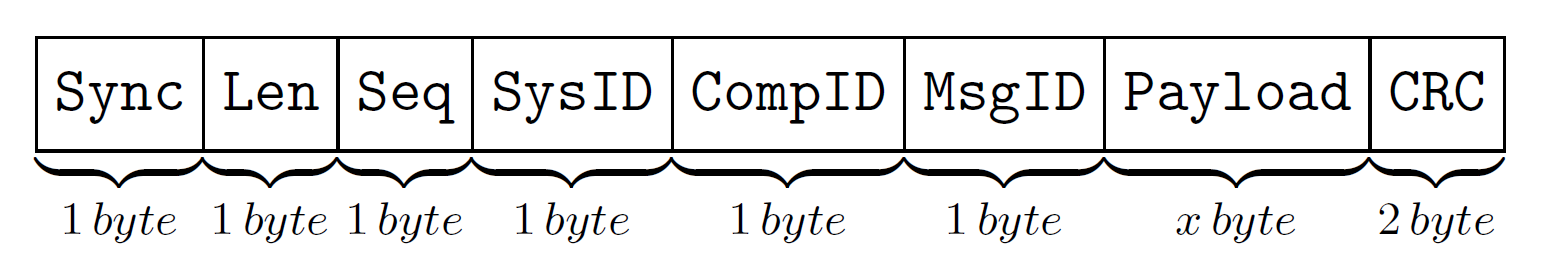
\includegraphics[width=0.75\textwidth]{Cap2/fig_message_structure}
\caption{Structure of a MAVLink v1.0 Message}
\label{fig_message_structure}
\end{figure}

A MAVLink message is a sequence of bytes encoded by a GCS and sent by telemetry over a wireless channel. In this process, the payload is transfomed into a specific data structure and sent in bytes through a channel followed by a checksum for error detection. The data structure of a message can be observed in the figure \ref{fig_message_structure}. The length of a message can vary from 8 to 263 bytes, according to the size of the payload. The fields of a message as shown in \ref{fig_message_structure} are:

\begin{itemize}
\item \textbf{Sync}: is a sequence that indicates the beginning of new MAVLink message. It is also known as protocol magic marker; 
\item \textbf{LEN}: indicates the length of the Payload;
\item \textbf{SEQ}: is the sequence number of the packet. It is used to detect packet loss;
\item \textbf{SysID}: identifies the sending system. It is used to differentiate diferent drones on the same network;
\item \textbf{CompID}: identifies the sending component inside a sending system;
\item \textbf{MsgID}: is the identification of the message, which is used to know how the payload must be interpreted;
\item \textbf{Payload}: data of the message, which contains the parameters. It is no longer than 255 bytes; 
\item \textbf{CRC}: is a 2 bytes checksum used for validation.
\end{itemize}

%The content of this section is based on the documentation provided in the link https://mavlink.io/en/

\section{Differences between versions}

First of all, a MAVLink 2.0 message has more fields than the previous version. The new fields were designed to bring more flexibility and security to the protocol communication.

The new features of MAVLink 2.0 are:
%https://mavlink.io/en/guide/mavlink_2.html
\begin{itemize}
\item More than 256 message IDs (24 bit message ID - over 16 million packets)
	In the version 1.0, only one byte was designed to message IDs  
\item Packet signing (authentication)
\item Extending existing MAVLink messages
\item Variable length arrays (simplified implementation).
\end{itemize}


\section{Working with XML}
MAVLink messages are defined in XML files. The messages that are common to all systems are defined in common.xml and only messages contained in this file are considered standard messages. 
%https://mavlink.io/en/messages/

\section{Adding a new message}

%http://ardupilot.org/dev/docs/code-overview-adding-a-new-mavlink-message.html

Adding a new message to the protocol can be done by following the steps. We will add a new message called NAMEOFMESSAGE to exemplify the tutorial.

\textbf{Step 1:} Install MAVProxy and the lastest version of ArduPilot code.

In section \ref{downloading_the_code} you can find how to clone the code from GitHub. Also check Mavproxy, which can be updated by running the next command line in a Terminal.

\begin{verbatim}
sudo pip install --upgrade mavproxy
\end{verbatim}

\textbf{Step 2:} Decide what type of message you want to add and how it will fit in with the existing MAVLink messages.

\textbf{Step 3:} Add the new message definition to the common.xml or ardupilotmega.xml file in the mavlink submodule;

%\textbf{Step 4:}

\textbf{Step 4:} Add functions to the main vehicle code to handle sending or receiving the command to/from the ground station. 


%%\begin{table}
%%\caption{Exemplo de uma Tabela}
%%\label{minhatab}
%\center
%\begin{tabular}{cccc}
 %  after \\: \hline or \cline{col1-col2} \cline{col3-col4} ...
 %\hline
%	Parametro & Unidade & Valor da simulação & Valor experimental   \\
%	\hline
 % Comprimento, $\alpha$ & $m$ &  $8,23$  & $8,54$ \\
  %Altura, $\beta$ & $m$     &  $29,1$ & $28,3$\\
	%Velocidade, $v$ & $m/s$  &  $60,2$ & $67,3$\\
	%\hline
%\end{tabular}
%\end{table}





